\documentclass[letter]{article}

%% Language and font encodings
\usepackage[english]{babel}
\usepackage[utf8x]{inputenc}
\usepackage[T1]{fontenc}
\usepackage{enumitem}
\usepackage{fancyhdr}
\pagestyle{fancy}

%% Useful packages
\usepackage{amsmath, amsthm, amssymb}
\usepackage{graphicx}
\newtheoremstyle{case}{}{}{}{}{}{:}{ }{}
\theoremstyle{case}
\newtheorem{case}{}


\title{HW3}
\author{Nicholas Silva Tee}
\lhead{Homework 3}



\begin{document}

\subsection*{Problem 1 Report}
This is the accuracy I got when using the given percentages of training data: \\
1\%(5 instances) = 76\% accuracy\\
2\%(10 instances) = 78\% accuracy\\
5\%(23 instances) = 78\% accuracy\\
10\%(45 instances) = 86\% accuracy\\
20\%(90 instances) = 88\% accuracy\\
100\%(450 instances) = 98\% accuracy\\
\begin{figure}[h!]
	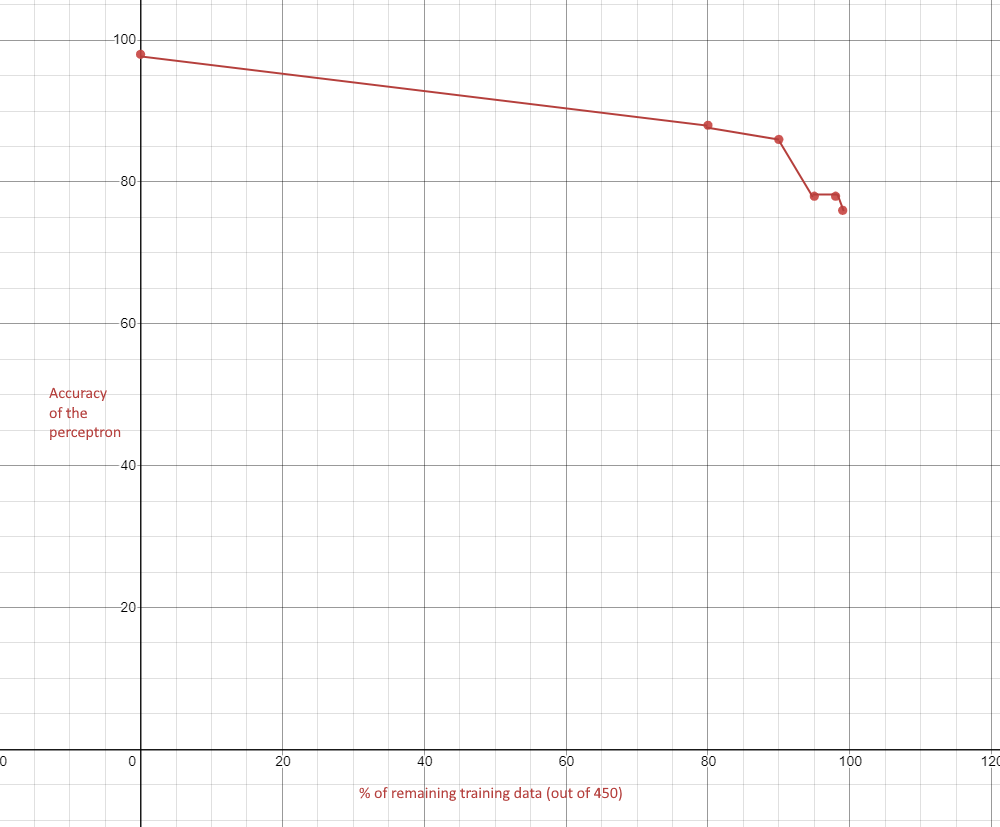
\includegraphics[scale=0.4]{accPlot.png}
\end{figure} 
\newpage
\subsection*{Problem 2 Report}
For testing the kNN classifier I used 10\% of the training data for testing. Since that means 4 instances as testing I took 1 from each of the labels \{1,2,3,4\}. As I increase the value of k these are the accuracies that I got.
\begin{table}[!h]
\begin{tabular}{|l|l|}
\hline
\multicolumn{1}{|c|}{k} & Accuracy \\ \hline
1                       & 4/4      \\ \hline
2                       & 2/4      \\ \hline
3                       & 4/4      \\ \hline
4                       & 3/4      \\ \hline
5                       & 3/4      \\ \hline
6                       & 3/4      \\ \hline
7                       & 3/4      \\ \hline
8                       & 2/4      \\ \hline
9                       & 2/4      \\ \hline
\end{tabular}
\end{table}
as k increases the accuracy slowly decreases as well. 

\end{document}










